%%%%%%%%%%%%%%%%%%%%%%%%%%%%%%%%%%%%%%%%%
% Beamer Presentation
% LaTeX Template
% Version 1.0 (10/11/12)
%
% This template has been downloaded from:
% http://www.LaTeXTemplates.com
%
% License:
% CC BY-NC-SA 3.0 (http://creativecommons.org/licenses/by-nc-sa/3.0/)
%
%%%%%%%%%%%%%%%%%%%%%%%%%%%%%%%%%%%%%%%%%

%----------------------------------------------------------------------------------------
%	PACKAGES AND THEMES
%----------------------------------------------------------------------------------------

\documentclass{beamer}
\usepackage{subfig}
\usepackage{pgfplots}

\mode<presentation> {

% The Beamer class comes with a number of default slide themes
% which change the colors and layouts of slides. Below this is a list
% of all the themes, uncomment each in turn to see what they look like.

%\usetheme{default}
%\usetheme{AnnArbor}
%\usetheme{Antibes}
%\usetheme{Bergen}
%\usetheme{Berkeley}
%\usetheme{Berlin}
%\usetheme{Boadilla}
%\usetheme{CambridgeUS}
%\usetheme{Copenhagen}
%\usetheme{Darmstadt}
%\usetheme{Dresden}
%\usetheme{Frankfurt}
%\usetheme{Goettingen}
%\usetheme{Hannover}
%\usetheme{Ilmenau}
%\usetheme{JuanLesPins}
%\usetheme{Luebeck}
\usetheme{Madrid}
%\usetheme{Malmoe}
%\usetheme{Marburg}
%\usetheme{Montpellier}
%\usetheme{PaloAlto}
%\usetheme{Pittsburgh}
%\usetheme{Rochester}
%\usetheme{Singapore}
%\usetheme{Szeged}
%\usetheme{Warsaw}

% As well as themes, the Beamer class has a number of color themes
% for any slide theme. Uncomment each of these in turn to see how it
% changes the colors of your current slide theme.

%\usecolortheme{albatross}
%\usecolortheme{beaver}
%\usecolortheme{beetle}
%\usecolortheme{crane}
%\usecolortheme{dolphin}
%\usecolortheme{dove}
%\usecolortheme{fly}
%\usecolortheme{lily}
%\usecolortheme{orchid}
%\usecolortheme{rose}
%\usecolortheme{seagull}
%\usecolortheme{seahorse}
%\usecolortheme{whale}
%\usecolortheme{wolverine}

%\setbeamertemplate{footline} % To remove the footer line in all slides uncomment this line
%\setbeamertemplate{footline}[page number] % To replace the footer line in all slides with a simple slide count uncomment this line

%\setbeamertemplate{navigation symbols}{} % To remove the navigation symbols from the bottom of all slides uncomment this line
}

\usepackage{graphicx} % Allows including images
\usepackage{booktabs} % Allows the use of \toprule, \midrule and \bottomrule in tables

\usepackage[USenglish,UKenglish,french,spanish,italian]{babel}
\usepackage[nodayofweek,level]{datetime}

\newcommand{\mydate}{\formatdate{22}{9}{2021}}
%----------------------------------------------------------------------------------------
%	TITLE PAGE
%----------------------------------------------------------------------------------------

\title[Fashion recommender systems]{Fashion recommender systems with focus on time and 
        seasonability} % The short title appears at the bottom of every slide, the full title is only on the title page

\author{Jaime Ferrando Huertas} % Your name
% \institute[H\&M] % Your institution as it will appear on the bottom of every slide, may be shorthand to save space
{

\medskip
% \textit{john@smith.com} % Your email address
}
\date{\mydate} % Date, can be changed to a custom date

\begin{document}

\selectlanguage{USenglish}
\begin{frame}
\titlepage % Print the title page as the first slide
\end{frame}

\begin{frame}
\frametitle{Overview} % Table of contents slide, comment this block out to remove it
\tableofcontents % Throughout your presentation, if you choose to use \section{} and \subsection{} commands, these will automatically be printed on this slide as an overview of your presentation
\end{frame}

%----------------------------------------------------------------------------------------
%	PRESENTATION SLIDES
%----------------------------------------------------------------------------------------

%------------------------------------------------
\section{Introduction} % Sections can be created in order to organize your presentation into discrete blocks, all sections and subsections are automatically printed in the table of contents as an overview of the talk
%------------------------------------------------
\begin{frame}{Introduction}
\begin{columns}[c] % The "c" option specifies centered vertical alignment while the "t" option is used for top vertical alignment

\column{.65\textwidth} % Left column and width
\begin{itemize}
\item Master Thesis collaboration with H\&M.
\item 40\% increase in online revenue from 2019 to 2020, with a total of 5.1 Billion euros. Highly susceptible for improvements on recommender systems
\item Fashion industry - different scenario as seen in state of the art recommender systems.
\end{itemize}

\column{.3\textwidth} % Right column and width 
\begin{figure}%
    \centering
    \centering{{
\includegraphics[scale=0.07]{images/1200px-H&M-Logo.svg.png} }}%
    % \caption{2 Figures side by side}%
\end{figure}
\end{columns}
\end{frame}

\begin{frame}{Introduction - Research question}

\begin{itemize}
\item Does treating our user's history as an ordered sequenced of events improve our recommendation models?
\end{itemize}
\end{frame}

\begin{frame}{Introduction - State of the art}

\begin{figure}[!htb]
\minipage{0.25\textwidth}
  
\includegraphics[width=\linewidth, scale=0.3]{images/spotifylogo.png}
\endminipage\hfill
\minipage{0.32\textwidth}
  
\includegraphics[width=\linewidth]{images/youtubelogo.png}
\endminipage\hfill
\minipage{0.32\textwidth}%
  
\includegraphics[width=\linewidth]{images/ALIBABA-LOGO.png}
\endminipage
\end{figure}
\begin{itemize}
\item Usage of Deep Learning methods across big tech companies. Models very closed to what is used in NLP.
\end{itemize} 

\end{frame}

\section{Dataset}
\begin{frame}{Dataset}
\begin{itemize}
    \item User interactions in H\&M website. Clicks, views.
    \item Swedish Market
    \item 1 month data, 2021-03-01 to 2021-04-01.
    \item Removed consecutive duplicates.
    \item Last user interactions as test set.
\end{itemize}
\end{frame}

\begin{frame}{Dataset - Preprocessing}
Given a user history $H$ containing $h_1, h_2, .. h_n$ interactions, a training sample can be created from each interaction, $h_t$ where the past interactions $h_1, .., h_t-1$ are used as past history to predict interaction $h_t$

\begin{columns}[c] % The "c" option specifies centered vertical alignment while the "t" option is used for top vertical alignment

\column{.25\textwidth} % Left column and width
\begin{figure}%
    \centering
    \centering{{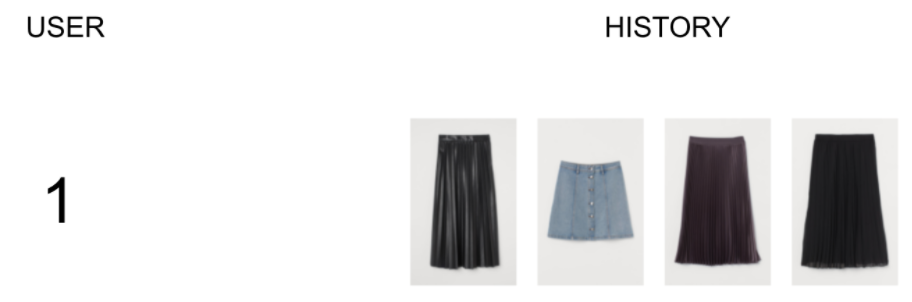
\includegraphics[scale=0.12]{images/dataset/dataset.png} }}%
    % \caption{2 Figures side by side}%
\end{figure}

\column{.5\textwidth} % Right column and width 
\begin{figure}%
    \centering
    \centering{{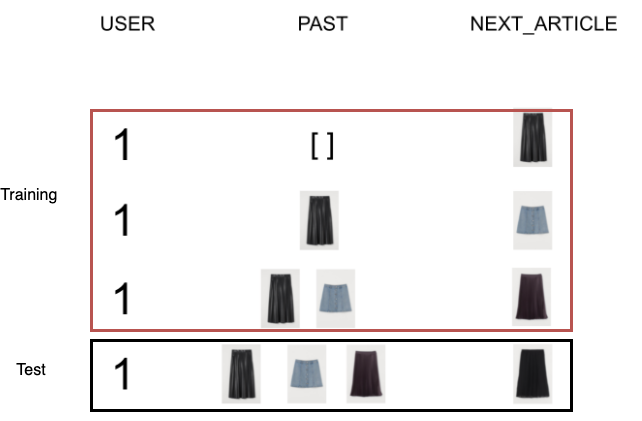
\includegraphics[scale=0.25]{images/dataset/datasetsplit.png} }}%
    % \caption{2 Figures side by side}%
\end{figure}
\end{columns}
Given $H$ the model will produce the conditional probability of the next item the user will interact across all different item classes. The ordered list of probabilities will represent the recommendation output from the model.

\end{frame}


\section{Evaluation}
\begin{frame}{Evaluation}
\begin{block}{Classification Performance}
\begin{itemize}
    \item Hit Ratio at K - Is the next interaction in the user recommendations set.
\end{itemize}
\end{block}

\begin{block}{Diversity}
\begin{itemize}
\item Coverage at K- \% of total items included in the recommendation set
\item Overlap at K- \% of user recommendations sets that are equal
\item Personalization at K - Measures how unique are each user recommendation set.
\item Novelty at K - Measures novelty of recommended items.
\end{itemize}
\end{block}   
At K: Measure within the top K recommendations. We will use 14.
\end{frame}

\section{Models}
\begin{frame}{Models}
\begin{columns}[c] % The "c" option specifies centered vertical alignment while the "t" option is used for top vertical alignment

\column{.5\textwidth} % Left column and width

\begin{figure}%
    \centering
    \centering{{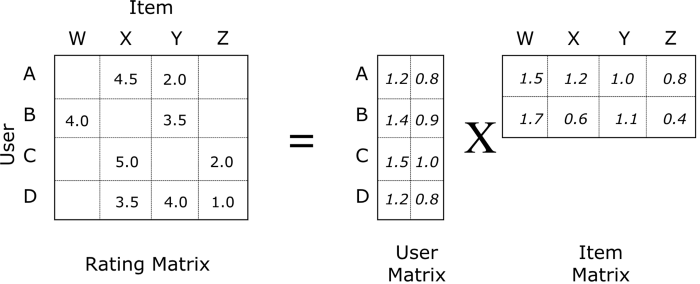
\includegraphics[scale=0.25]{images/background/matrix_factorization.png} }}%
    % \caption{2 Figures side by side}%
\end{figure}
\vspace{30px}
\begin{itemize}
    \item AALS - Aproximate Alternative Least Squares 
\end{itemize}

\column{.45\textwidth} % Right column and width 

\begin{figure}%
    \centering
    \centering{{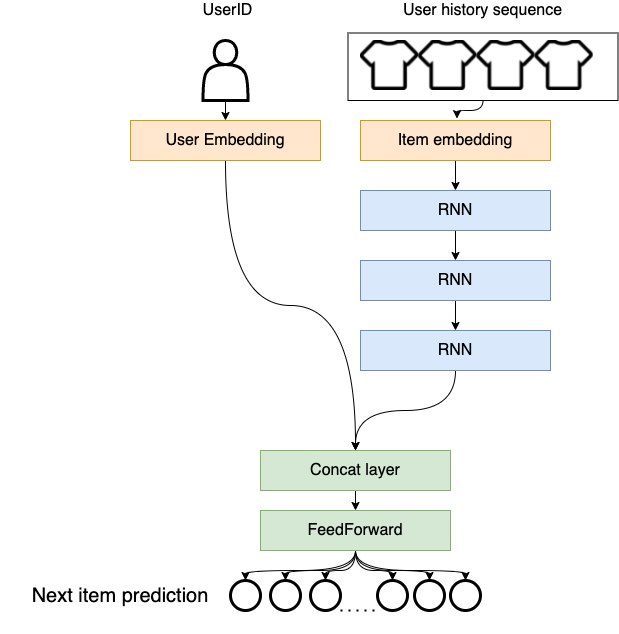
\includegraphics[scale=0.2]{images/models/RNN.png} }}%
    % \caption{2 Figures side by side}%
\end{figure}

\begin{itemize}
    \item Neural Sequencer - Tried RNN, LSTM, GRU, Attention, Transformers
\end{itemize}
\end{columns}

\end{frame}



\section{Experiments}
\begin{frame}{Experiments - Models performance}
\begin{table}[H]
\begin{tabular}{|l|r|r|r|r|r|}
\hline
\multicolumn{1}{|c|}{\textit{Experiments}} & \multicolumn{1}{c|}{\textit{\begin{tabular}[c]{@{}c@{}}HR\\ @14\end{tabular}}} & \multicolumn{1}{c|}{\textit{\begin{tabular}[c]{@{}c@{}}Coverage\\ @14\end{tabular}}} & \multicolumn{1}{c|}{\textit{\begin{tabular}[c]{@{}c@{}}Overlap\\ @14\end{tabular}}} & \multicolumn{1}{c|}{\textit{\begin{tabular}[c]{@{}c@{}}Personalization\\ @14\end{tabular}}} & \multicolumn{1}{c|}{\textit{\begin{tabular}[c]{@{}c@{}}Novelty\\ @14\end{tabular}}} \\ \hline
AALS                                       & 4.42\%                                                                         & 0.24\%                                                                               & {\color[HTML]{333333} \textbf{14.45\%}}                                             & 56.81\%                                                                                     & 7.6                                                                                 \\ \hline
N.S LSTM                                   & \textbf{50.32\%}                                                               & \textbf{8.75\%}                                                                      & {\color[HTML]{333333} 21.54\%}                                                      & \textbf{90.57\%}                                                                            & \textbf{9.88}                                                                       \\ \hline
N.S RNN                                    & 43.94\%                                                                        & 7.68\%                                                                               & {\color[HTML]{333333} 19.84\%}                                                      & 89.87\%                                                                                     & 9.51                                                                                \\ \hline
N.S GRU                                    & 49.00\%                                                                        & 8.04\%                                                                               & {\color[HTML]{333333} 25.94\%}                                                      & 88.03\%                                                                                     & 9.45                                                                                \\ \hline
N.S Attention                              & 47.46\%                                                                        & 7.61\%                                                                               & {\color[HTML]{333333} 19.84\%}                                                      & 89.55\%                                                                                     & 9.44                                                                                \\ \hline
N.S Transformer                            & 44.33\%                                                                        & 7.67\%                                                                               & 21.97\%                                                                             & 86.98\%                                                                                     & 9.36                                                                                \\ \hline
\end{tabular}
\caption{Model results overview} \label{faketable:mul}
\end{table}
\end{frame}

\begin{frame}{Experiments - Embeddings}

\begin{table}[H]
\resizebox{\textwidth}{!}{\begin{tabular}{|l|l||r|r|r|r|r|}
\hline
\textit{User Size} & \multicolumn{1}{c||}{\textit{Item Size}} & \multicolumn{1}{c|}{\textit{\begin{tabular}[c]{@{}c@{}}HR\\ @14\end{tabular}}} & \multicolumn{1}{c|}{\textit{\begin{tabular}[c]{@{}c@{}}Coverage\\ @14\end{tabular}}} & \multicolumn{1}{c|}{\textit{\begin{tabular}[c]{@{}c@{}}Overlap\\ @14\end{tabular}}} & \multicolumn{1}{c|}{\textit{\begin{tabular}[c]{@{}c@{}}Personalization\\ @14\end{tabular}}} & \multicolumn{1}{c|}{\textit{\begin{tabular}[c]{@{}c@{}}Novelty\\ @14\end{tabular}}} \\ \hline
1                  & 256                                     & 49.35\%                                                                        & 8.67\%                                                                               & 23.88\%                                                                             & 89.84\%                                                                                     & 9.87                                                                                \\ \hline
256                & 256                                     & \textbf{50.32\%}                                                                        & \textbf{8.75\%}                                                                               & \textbf{21.54\%}                                                                    & \textbf{90.57\%}                                                                            & \textbf{9.88}                                                                          \\ \hline
\end{tabular}}
\caption{User embedding size study on N.S LSTM}
\end{table}

\begin{table}[H]
\resizebox{\textwidth}{!}{\begin{tabular}{|l|l||r|r|r|r|r|}
\hline
\textit{User Size} & \multicolumn{1}{c||}{\textit{Item Size}} & \multicolumn{1}{c|}{\textit{\begin{tabular}[c]{@{}c@{}}HR\\ @14\end{tabular}}} & \multicolumn{1}{c|}{\textit{\begin{tabular}[c]{@{}c@{}}Coverage\\ @14\end{tabular}}} & \multicolumn{1}{c|}{\textit{\begin{tabular}[c]{@{}c@{}}Overlap\\ @14\end{tabular}}} & \multicolumn{1}{c|}{\textit{\begin{tabular}[c]{@{}c@{}}Personalization\\ @14\end{tabular}}} & \multicolumn{1}{c|}{\textit{\begin{tabular}[c]{@{}c@{}}Novelty\\ @14\end{tabular}}} \\ \hline
256                                      & 1                                       & 35.54\%                                                                        & 6.20\%                                                                               & 22.80\%                                                                             & 89.40\%                                                                                     & 9.8 \\ \hline
256                                      & 256                                     & \textbf{50.32}\%                                                                        & \textbf{8.75\%}                                                                      & \textbf{21.54\%}                                                                             & \textbf{90.57\% }                                                                                    & \textbf{9.88}                                                                        \\ \hline
\end{tabular}}
\caption{Item embedding size study on N.S LSTM}
\end{table}
\end{frame}

\begin{frame}{Experiments - Ordering}

\begin{table}[H]
\begin{tabular}{|r|r|r|r|r|r|}
\hline
\multicolumn{1}{|c|}{\textit{\begin{tabular}[c]{@{}c@{}}User history\\ Sequence order\end{tabular}}} & \multicolumn{1}{c|}{\textit{\begin{tabular}[c]{@{}c@{}}HR\\ @14\end{tabular}}} & \multicolumn{1}{c|}{\textit{\begin{tabular}[c]{@{}c@{}}Coverage\\ @14\end{tabular}}} & \multicolumn{1}{c|}{\textit{\begin{tabular}[c]{@{}c@{}}Overlap\\ @14\end{tabular}}} & \multicolumn{1}{c|}{\textit{\begin{tabular}[c]{@{}c@{}}Personalization\\ @14\end{tabular}}} & \multicolumn{1}{c|}{\textit{\begin{tabular}[c]{@{}c@{}}Novelty\\ @14\end{tabular}}} \\ \hline
Correct order                                                                                        & \textbf{50.32\%}                                                               & \textbf{8.75\%}                                                                      & \textbf{21.54\%}                                                                    & \textbf{90.57\%}                                                                            & \textbf{9.88}                                                                       \\ \hline
Day level order                                                                                    & 49.37\%                                                                        & 8.04\%                                                                               & 23.39\%                                                                             & 90.46\%                                                                                     & 9.55                                                                                \\ \hline
Random                                                                                               & 43.37\%                                                                        & 7.73\%                                                                               & 22.89\%                                                                             & 85.41\%                                                                                     & 8.89                                                                                \\ \hline
\end{tabular}
\caption{User history sequence order study on N.S LSTM}
\end{table}
\end{frame}

\begin{frame}{Experiments - History}

\begin{table}[H]
\begin{tabular}{|r|r|r|r|r|r|}
\hline
\multicolumn{1}{|c|}{\textit{\begin{tabular}[c]{@{}c@{}}User history\\ Sequence order\end{tabular}}} & \multicolumn{1}{c|}{\textit{\begin{tabular}[c]{@{}c@{}}HR\\ @14\end{tabular}}} & \multicolumn{1}{c|}{\textit{\begin{tabular}[c]{@{}c@{}}Coverage\\ @14\end{tabular}}} & \multicolumn{1}{c|}{\textit{\begin{tabular}[c]{@{}c@{}}Overlap\\ @14\end{tabular}}} & \multicolumn{1}{c|}{\textit{\begin{tabular}[c]{@{}c@{}}Personalization\\ @14\end{tabular}}} & \multicolumn{1}{c|}{\textit{\begin{tabular}[c]{@{}c@{}}Novelty\\ @14\end{tabular}}} \\ \hline
5                                          & 45.00\%                                                                        & \textbf{8.77\%}                                                                               & 25.19\%                                                                             & 92.05\%                                                                                     & 9.41                                                                                \\ \hline
10                                         & 48.00\%                                                                        & 8.61\%                                                                               & 26.60\%                                                                             & 89.50\%                                                                                     & 9.25                                                                                \\ \hline
Default value - 20                         & 50.32\%                                                                        & 8.75\%                                                                      & 21.54\%                                                                             & 90.57\%                                                                                     & \textbf{9.88}                                                                       \\ \hline
50                                         & \textbf{50.35\%}                                                               & 7.78\%                                                                               & \textbf{16.76\%}                                                                    & \textbf{94.60\%}                                                                            & 9.69                                                                                \\ \hline
\end{tabular}
\caption{User history sequence length study on N.S LSTM}
\end{table}
\end{frame}



\section{Conclusions and future work}
\begin{frame}{Conclusions}

\begin{itemize}
    \item Neural models beat our baseline matrix factorization methods.
    \item User and item embeddings both play different roles and affect specific metrics. 
    \item It is not only the raw neural based models performance, but treating the user history as an ordered sequence that reports best results.
    \item The more history of the user we include, the better.
    \item Unable to follow NLP research path.
\end{itemize}
\end{frame}
%------------------------------------------------
\begin{frame}{Future work}
\begin{itemize}
    \item Recommendations longevity - Study model's performance over time, how quick it degrades.
    \item Transfer learning - Reuse embeddings and previous models.
    \item Split representation and recommendation models - Train each one separately first and then join them.
    \item Usage of item/user features with embeddings - Will help reduce cold starts.
\end{itemize}

\end{frame}

\begin{frame}
\Huge{\centerline{Questions}}
\end{frame}
%----------------------------------------------------------------------------------------

\end{document}